\chapter{低功耗海洋传感器集成系统总体设计方案}
本设计是使复杂的传感器系统小型化并降低设备成本的新方法。它们适度的尺寸和功耗也允许对系统的部署进行经济高效的设计。进行具有成本效益的部署的另一条途径是通过在单个平台上使用多个微型传感器。例如,PH值、温盐深和叶绿素等微型传感器同时部署在一个集成系统之中。同时其系统的稳定性使得系统可长期提供高质量的数据。

\section{系统的设计目标和总体框架}
\subsection{系统的设计目标}
海洋科学中目前正在追寻的重大科学问题所要求的在时间和空间的尺度上实现数据收集,要求我们对待海洋观测的方式发生了重大的转变。海洋科学与工程现在必须专注于大幅度降低传感器成本,并且增加许多生物、地球、化学和生物过程的高异质性有关的时空覆盖范围。在某种程度上,传感器的发展和部署已经开始具有成本效益,通常是由于实际传感器组件的成本和尺寸的减少而加速的。

本课题基于海洋科学研究和海洋环境安全保护的要求,以系统低功耗和高稳定性为目标,设计并实现了低功耗海洋传感器集成系统用于长期、定时获取海洋生态环境数据。低功耗海洋传感器集成系统与传统的海洋传感器集成系统相比,具有几方面的先进性和创新性:

1)自容性和低功耗:整个系统采用集成式部署方式,只有一个任务处理中心。在电路设计时,尽可能考虑其微型化。同时不需要外部的电源进行供电,锂电池串联的电池组作为接入电源。采用MSP430系列微处理器来对电源进行控制,通过定点启动电源来触发采集任务,当平台数据采集任务处于上一个工作周期与下一个工作周期的中间休眠期时,将关闭电源,使微处理器与传感器可以在间歇时刻休息,以此来进一步降低平台的功耗。

2)多接口、可拓展:除了微处理器本身硬件接口外,还对串口进行了拓展,使用了成都为开公司的串口扩展芯片WK2124进行了串口扩展,扩展如此之多的串口是因为所采用的传感器大多是基于串口协议进行通信的。

3)易替换:多种海洋传感器可以任意的进行替换,不需要再单独设计硬件电路。在几秒钟内无需工具的情况下,即可在海上更改传感器的类型。

4)支持两种通信协议:标准的RS232协议和AML传感器接口协议。

\subsection{系统的关键技术}
1)多种通信协议拓展电路以集成多类传感器设备并确保双向通信两端数据能安全可靠地无干扰传输。

2)利用升降平台将系统设备精准释放,使用水密舱保证系统的密闭性。

3)由于系统自携带电池式工作,且舱体的体积和重量受到一定的限制,为了确保整体系统在水下长时间稳定可靠的工作,需要通过软件和硬件的设计并完善整个系统的低功耗电源管理技术,减少携带的电池量,延长整个系统的生命周期。

4)海洋要素数据回收预留接口,不需要对水密舱进行拆卸,即可对系统采样的数据进行现场回收。

\section{系统整体框架设计}
低功耗海洋传感器集成系统的整体框架主要由传感器单元和微处理器单元组成。整个系统能够对海洋生态环境进行长期、定时的在线监测,系统整体框图如图~\ref{fig:系统框图}所示。

\begin{figure*}[ht]
    \centering
	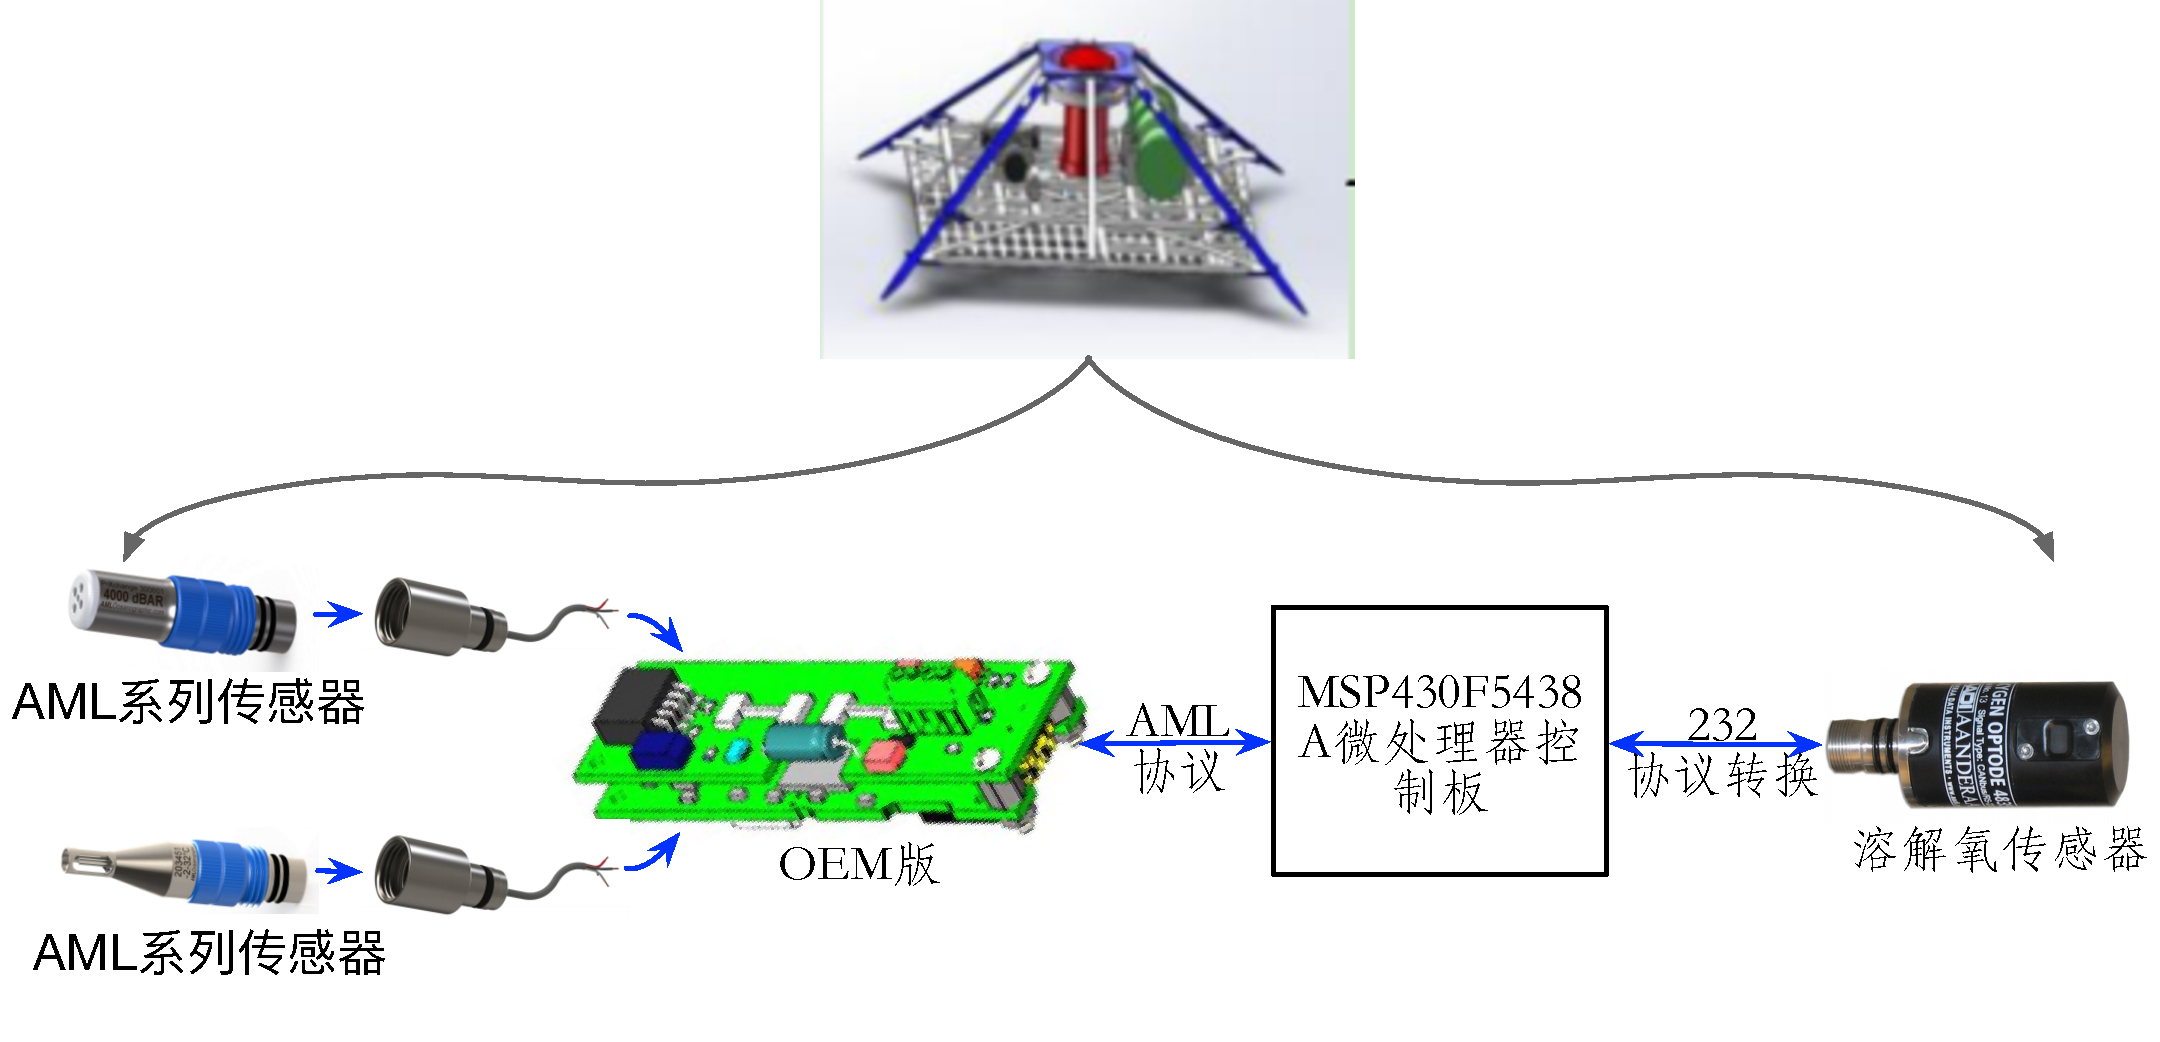
\includegraphics[width=1\textwidth]{fig/系统框图.pdf}
	\caption{海洋传感器集成系统整体架构图}
	\label{fig:系统框图}
\end{figure*}

传感器单元主要包括AML系列传感器和其他类型海洋传感器。AML系列传感器由于通信协议和接口都是一致的,通常它们可以互相替换,这些传感器通过OEM板与微处理器单元进行连接。其他类型的海洋传感器,比如溶解氧传感器等,通常是通过RS232或485协议与微处理器单元进行通信。微处理器单元主要包括MSP430F5438A为核心的最小系统和外围电路,比如用于传感器通信的协议转化电路、用于数据保存的存储电路等。

\section{系统硬件平台设计}
低功耗海洋传感器集成系统的硬件设计进行了多种海洋传感器的集成~\cite{2015cd},从而实现了对海洋生态环境数据的高效管理和采集。同时,还介绍了多个海洋传感器的特点和控制方法。作为一套较为完善且具有通用型的海洋传感器集成系统,后期还可能进行拓展集成。

不同的器件之间会存在供电电压的差异,使用相应供电电压的DC/DC转换器来解决电源供应问题,同时考虑到DC/DC电压转换模块的功率要求,以满足实际电路模块中的负载问题。

在系统设计中采用单处理器集中控制集成传感器,通过给传感器下达指令,完成数据采集等任务。考虑到系统的稳定性、可靠性以及后期的可拓展性,在数据通信模块中实现通信协议之间的转换,根据传感器数量对串口进行了相应的拓展。采用MSP430F5438A作为控制核心,它的作用至关重要,有超低的功耗和有良好的性能,同时拥有众多的接口资源。其中对于微处理器部分的设计框图如图~\ref{fig:微处理器}所示,传感器可以根据实际情况进行挂载或更换。
\begin{figure*}[ht]
    \centering
	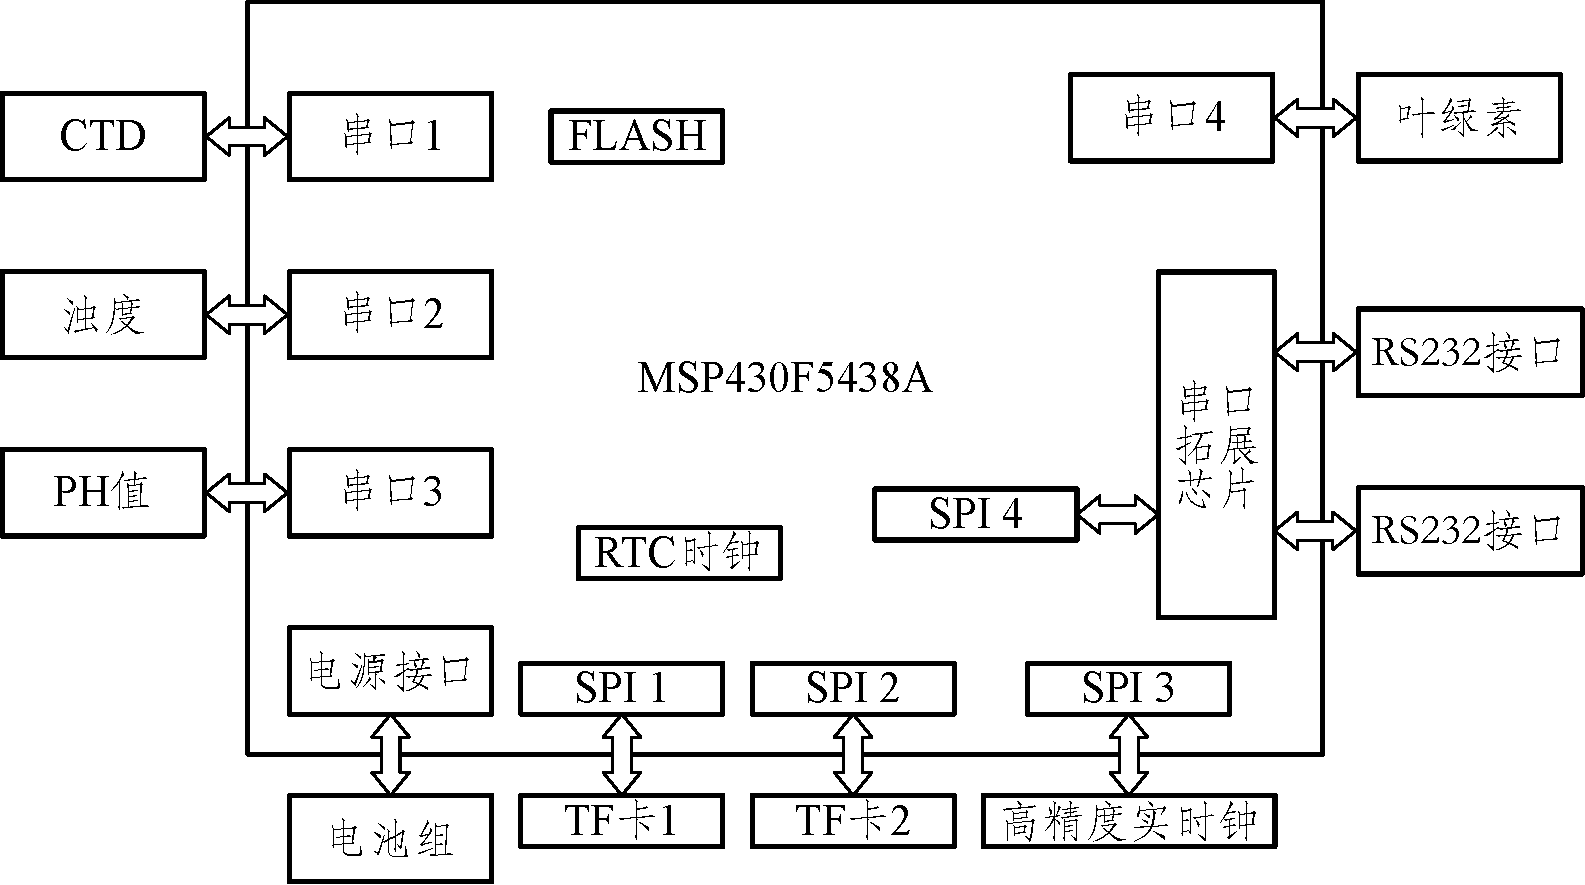
\includegraphics[width=1\textwidth]{fig/微处理器部分设计框图.pdf}
	\caption{微处理器部分设计框图}
	\label{fig:微处理器}
\end{figure*}

\section{系统软件平台设计}
低功耗海洋传感器集成系统的软件设计是整个系统设计环节的重要部分,只有高效、可靠的软件设计配合安全、可靠的硬件平台才能保证整个系统的稳定性。软件设计上实现传感器数据采集、数据存储、数据处理、数据回收等一系列操作,并在系统性能、微处理器资源配置、外设模块调度和软件逻辑框架上做大量研究,以保证系统以最低的功耗、最高的效率完成指定任务。软件平台分模块进行程序设计,通过系统管理与配置模块和数据采集与通信模块,分别实现与管理人员、海洋传感器之间的信息交互。能源管理与控制模块的软件设计实现了电源的有效控制,数据存储和回收模块对海洋生态数据进行有效的保存和处理。
\section{海洋传感器介绍}
在海洋观测与监测领域,海洋传感器被广泛应用于测量各种海洋环境因素,如温度、压力、深度等。电导率/盐度和其他基本物理参数海洋因素,对海洋资源的科学研究和开发具有重要意义。本文中海洋传感器需采集温度、深度、盐度、叶绿素、溶解氧、PH值、浊度、流速等海洋环境要素。

\subsection{AML多参数水质测量仪}
多参数水质测量仪可定点测量海洋各种生态环境要素,通过安装多个传感器探头即可采集不同的海洋要素。加拿大AML公司的AML Micro$\cdot$X传感器是一项重大进步在海洋仪器中。X代表是一个系列的海洋传感器,可依据现场状况和需要采集的海洋生态环境要素选择传感器负载。可交换和可互换的传感器极大地改善了海洋仪器多方面功能。在几秒钟内无需工具的情况下,即可在海上更改传感器的类型。例如,CTD可以通过更换传感器头将其更改为叶绿素分析器。为了优化传感器数据的分辨率和准确率,可以将传感器配置为可更改测量范围。

Micro$\cdot$X可以通过RS232或RS485串行连接进行通信。与传感器建立通信必须要使用正确的通信端口和设置。通信设置为8个数据位,1个停止位,无奇偶校验,无流量控制以及通信双方需同步波特率。波特率600、1200、2400、4800、9600、19200、或38400皆可以使用。当外部通信设备与传感器建立连接通信链路后就可以向传感器发送命令来完成状态显示、数据采集设置、数据检索和诊断测试工作。常用命令如下:

\begin{lstlisting}
SCAN:测量并输出一次数据扫描。
MONITOR:以设定的采样率进行扫描。
VERSION:显示仪器标识头。
DISPLAY OPTIONS:显示仪器状态和用户设置。
DISPLAY SAMPLE RATE:设置波特率。
\end{lstlisting}

Micro$\cdot$X传感器主要参数指标如表~\ref{tab:MicroX}所示。
\begin{table*}[h]
  \centering\small
  \caption{Micro$\cdot$X传感器参数表}
  \label{tab:MicroX}
\begin{tabular}{|c|c|c|}
\hline
\multirow{9}{*}{\bf 传感器测量范围和精度}      & 温度       & 范围: -5-45$^{\circ}$C  ,精度:  $\pm$ 0.003$^{\circ}$C          \\ \cline{2-3} 
                                           & 压力       & 范围: 
 50-6000dBar , 精度: $\pm$ 0.3\%FS                 \\ \cline{2-3} 
                                           & 盐度       & 范围:
0-42psu, 精度:$\pm$ 0.003psu              \\ \cline{2-3} 
                                           & 叶绿素      & 范围:
0-250ug/l,精度:   $\pm$ 0.2\%FS            \\ \cline{2-3} 
                                           & 浊度       & 范围 :
0-3000NTU,精度:   $\pm$ 0.5\%NTU         \\ \cline{2-3} 
                                           & PH       & 范围 :
0-14[PH],精度:$\pm$ 0.01[PH]             \\ \cline{2-3} 
                                           & 溶解氧      & 范围:
0-25mg/l,精度:$\pm$ 0.01mg/l               \\ \cline{2-3} 
                                           & 声速       & 范围 :
1375-1625m/s,精度:$\pm$ 0.006m/s           \\ \cline{2-3} 
                                           & 电导率      & 范围:
0-90mS/cm,精度:$\pm$0.003mS/cm            \\ \hline
\multicolumn{2}{|c|}{采样间隔}                  & 10min(设定)                         \\ \hline
\multicolumn{2}{|c|}{通信协议}                  & \multicolumn{1}{c|}{RS232/RS485}       \\ \hline
\end{tabular}
\end{table*}


\subsection{声学波浪流速剖面仪}
声学波浪流速剖面仪主要是用来测量波浪、流速剖面、方向波谱等海洋数据的传感器,简称AWAC,是一种适应性强且工作稳定的海洋监控设备。本文所讲的AWAC是基于挪威Nortek公司的产品来进行描述的~\cite{foteinis2017comparative},其工作原理主要依据多普勒效应,即在水中发送出一个短脉冲声波,在水中遇到障碍物时将会产生回音和频率的变化,据此数据对比用来测量水流的速度,同时还可以利用该传感器测量多种波浪数据~\cite{2016xcc}。

AWAC不仅可以实现使用内置电池和存储器的自容测量,还可以实现系统的在线观测。AWAC一般需要相应的挂载平台,一方面用于固定设备,另一方面可以减少外界对设备的损伤,为了防止设备生锈腐蚀,AWAC使用全塑料和钛合金材料制作外壳,使用钛合金材料不仅可以增大设备的看腐蚀性,还可以增大设备的耐压性。

\begin{table*}[htb]
  \centering\small
  \caption{AWAC技术指标和命令}
  \label{tab:AWAC}
\begin{tabular}{|c|c|c|}
\hline
\multicolumn{2}{|c|}{\bf 技术参数}                  &{\bf 性能指标 }                        \\ \hline
\multicolumn{2}{|l|}{工作频率}                  & \multicolumn{1}{l|}{10min流速剖面,1h波浪}                \\ \hline
\multicolumn{2}{|l|}{声学频率}                  & \multicolumn{1}{l|}{1MHz/600kHz/400kHz}                \\ \hline
\multicolumn{2}{|l|}{流速范围}                  & \multicolumn{1}{l|}{水平方向$\pm$10 m/s,光束方向$\pm$5 m/s}                         \\ \hline
\multicolumn{2}{|l|}{剖面范围}                  & \multicolumn{1}{l|}{30-40m}                     \\ \hline
\multicolumn{2}{|l|}{深度单元}                  & \multicolumn{1}{l|}{典型20-40层,最大128层}                       \\ \hline
\multicolumn{2}{|l|}{测量精度}                  & \multicolumn{1}{l|}{测量值的1\%或$\pm$0.5cm/s}                        \\ \hline
\multicolumn{2}{|c|}{\multirow{2}{*}{常用命令}} & \multicolumn{1}{l|}{Break-是仪器中断再重新启动}     \\ \cline{3-3} 
\multicolumn{2}{|l|}{}                          & \multicolumn{1}{l|}{ST-采样命令,串口输出数据} \\ \hline
\end{tabular}
\end{table*}

AWAC 有多种数据格式,如信息设置、传感器数据、流速数据、波浪特征参 数数据、波能量密度谱、波带特征参数、波浪傅里叶系数波谱~\cite{2014wjs}。在完成设备的基本设置后便可执行数据采集的工作,其相关技术参数如表格~\ref{tab:AWAC}所示。

\subsection{浊度传感器}
浊度传感器主要用来检测海水中悬浮物和胶状体对光线透过时所产生的阻碍程度,表征水样的光学性质,将依据悬浮物在水中存在漫反射等特性使用浊度传感器来检测水体的浑浊程度~\cite{2015wj}。主要是把水样的浊度转换为光电信号来进行检测,进而计算得出浊度值,具体可分为透射法、散射法等。

在本文中所使用的浊度仪器为美国Wetlabs公司所生产ECO-NTU浊度计,其表面采用具有自清洁功能的纳米防污材料,能够在海水环境中工作数月。并且具有耐腐蚀强、尺寸小、受光线影响小等优点,能够应用于海洋监测。相关技术参数如表格~\ref{tab:ECO-NTU}所示。

\begin{table}[htb]
  \centering\small
  \caption{ECO-NTU技术指标和命令}
  \label{tab:ECO-NTU}
\begin{tabular}{|c|c|c|}
\hline
\multicolumn{2}{|c|}{\bf 技术参数}                  & {\bf 性能指标}                         \\ \hline
\multicolumn{2}{|l|}{工作波长}                  & \multicolumn{1}{|c|}{700nm}                \\ \hline
\multicolumn{2}{|l|}{测量范围}                  & \multicolumn{1}{c|}{可选0-70NTU、0-200NTU、0-1000$\mu$g/L}                \\ \hline
\multicolumn{2}{|l|}{采样频率}                  & \multicolumn{1}{c|}{8Hz}                         \\ \hline
\multicolumn{2}{|c|}{波特率}                  & \multicolumn{1}{c|}{19200 baud}                     \\ \hline
\multicolumn{2}{|l|}{深度范围}                  & \multicolumn{1}{c|}{0-20/200$\mu$g/L}                       \\ \hline
\multicolumn{2}{|l|}{测量精度}                  & \multicolumn{1}{c|}{0.02$\mu$g/L}                        \\ \hline
\multicolumn{2}{|c|}{\multirow{2}{*}{常用命令}} & \multicolumn{1}{c|}{RUN-开始工作}     \\ \cline{3-3} 
\multicolumn{2}{|l|}{}                          & \multicolumn{1}{c|}{MVS-Bio刷开始/关闭} \\ \hline
\end{tabular}
\end{table}


\subsection{UV紫外灯}

在深海的环境进行长期的在线观测,海洋微生物的附着和海洋生物对设备的撞击都会影响到观测系统的正常运行。在过去十年中已经解决了对传感器的感测区域的保护的问题。比如,为了避免这些情况,往往会在观测系统中添加UV紫外灯。从而可以有效地防止生物污染。这将减少维护成本,提高收集数据的质量(减少与生物污损有关的干扰),并避免在环境中不必要地引入潜在有害的化学物质。
本系统采用AML公司的UV\_Xchange,它利用紫外线防止藻类及其他微生物生长在传感器的表面。UV光源光谱范围是200nm-450nm,以365nm为中心,光源可以有效防止微生物对水下设备的附着。UV紫外灯实物如图~\ref{fig:UV}所示。

\begin{figure*}[ht]
    \centering
	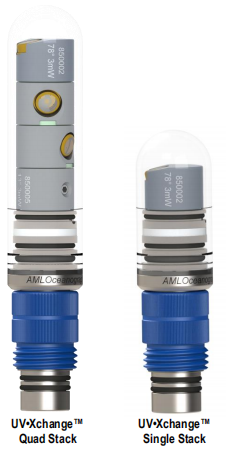
\includegraphics[width=0.3\textwidth]{fig/UV灯.png}
	\caption{UV紫外灯}
	\label{fig:UV}
\end{figure*}

\subsection{溶解氧传感器}
本系统采用安德拉公司的Oxygen Optode4835传感器。由于氧气参与了大多数水生生物和化学过程,所以氧气在海洋研究中可以作为一种示踪器。安德拉系列的溶解氧传感器具有长期稳定、受压力影响小、响应时间快等优点。设备可使用CAN总线或者RS-232总线与传感器进行连接,可以获取氧气的浓度、饱和度和温度。

Oxygen Optode 4835传感器的主要工作指令如下所示:
\begin{lstlisting}
"/"或";"(英文状态)指令      ******唤醒传感器
start指令                     *******传感器开始采集数据
stop指令                      ******传感器停止采集数据
measurement指令               ******传感器采集数据反馈
save指令                      ******保存传感器配置
\end{lstlisting}

\section{本章小结}
在本章节中对低功耗海洋传感器集成系统的整体架构进行了分体介绍,简略讲述了各部分的结构组成,并对其中每部分的独立功能进行了介绍,以论述海洋观测系统中各部分之间的组成关系以及工作关系,同时对传感器的性能指标做了简要概述。